\section{Premise}

The premise of this treatise is that it must be possible to create
a binary encoding format specification such that any random input 
deterministically and without an error, produces a valid output.
The use of this specification must allow for complex data structures
in the output of the decoder (for example, as offered by ASN.1 \cite{bib:asn1}
  XML \cite{bib:xml} or JSON \cite{bib:json}).

In other words, the following should always work:

\begin{changemargin}{-60mm}{0mm}
\begin{myquote}
\begin{verbatim}

$ cat /dev/random | head -c $ANYNUMBER > /tmp/foo
$ ./decoder < /tmp/foo
$ #... some convoluted, incomprehensible JSON expression on stdout...

\end{verbatim}
\end{myquote}
\end{changemargin}

\section{Problem Statement}

Binary encodings are often chosen because of their density.
However, when applied, they usually contain at least some 'air'
(superfluous or useless information).
The problem with binary encodings is that this 'air' can also contain
encoding mistakes. For example:

\begin{itemize}
\item When using TLV \cite{bib:tlv}, they may contain undefined type identifiers.
\item When using TLV, they may contain lengths that are illegal.
  Either because they are zero, which the type does not support,
  or because they exceed the length of the message size, or
  the size of the element that contains them.
\item For example, in DER \cite{bib:ber} encoding it is possible to define lengths
  that could not possibly exist in our universe.
\item For example, in UTF-8, there exist illegal wide character encodings.
\end{itemize}

Textual formats can convey complex data structures, but are also
(very) error prone. For example:

\begin{itemize}
\item String escaping may lead to illegal escape sequences or breaking
  of string enclosing logic.
\item Closing strings and brackets may be ommitted or over-supplied.
\item Closing tags - same thing.
\item 8-bit relevant bytes in 7-bits clean messages encoded as 8-bit formats.
\end{itemize}
etc.

All of these formats are problematic because we have to deal with
errors during parsing. Errors in parsing are hardly ever meaningful,
since we have no good way to recover from them (but they do introduce
a lot of extra code). The most we can usually do, is point out where
grammar was broken. Error correcting codes can be provided with any input,
but they don't fix 'honest mistakes' - just error(s) in transmission.

Tail end recovery of both 'JSON'- or 'DER'-like encodings should be
relatively easy (just wrap up the parsing effort and present the current
state of the parser as the result to the caller), but this is not standard.
With the content encoding format described in this paper however, tail end
recovery is implicit.

\section{Design Principles}
 
\begin{itemize}
\item Length can never be used in the way that it may be used to 
  under- or overflow the message or message segment size.
\item Our atom will be a bit, not a byte, as we cannot have any 'air'
  in our encoding.
\item Complexity of the output must be 'like ASN.1, XML or JSON'.
  That is to say:
  \begin{itemize}
  \item Encodes all eight-bit bytes and all lengths of those bytes.
        And maybe even wide characters.
  \item Is complex in that it provides at least for nulls, booleans,
        strings, integers,
        floating points, 'hashtable' name-value lists, and arrays.
        Optionally, the type system is extensible.
  \end{itemize}
\item We don't care about being truly efficient. The fact that we're
  binarily encoding should bring us enough of that. The main goal stands:
  any decoder input must produce an output.
\item We don't care about deterministic reciprocity between encoding
  and decoding: if the input to the decoder produces
  a complex data structure, then the complex data structure, when fed
  to the encoder, doesn't need to produce a copy of the input.
\item There exists a 'null' type, which can be given explicitly, or
  we use it to fill in all sorts of blanks.
\item On top, everything is implicitly inside a list.
  When the implicit list contains
  one element, it is a scalar. If you want to define a list with
  one element, you must explicitly define a list.
\item At the end of input, however many zero bits as are required can be read.
  Since all reads are implicitly length delimited ('next byte' in string 
  reading never pops more than nine bits, integers pop 64 bits, etc),
  this is a one-time affair only. All loops (strings, hashtables, arrays)
  take the end of input as to mean: jump out of the loop and return.
\end{itemize}

\section{Specification}

Explicitly written from the standpoint of the decoder.
The encoder will use this specifiction simply in reverse.

\begin{itemize}
\item There are the following types (eight, so that they fit exactly
      into three bits):
  \begin{itemize}
  \item Implicit NULL
  \item Explicit NULL
  \item BOOLEAN
  \item INTEGER (64 bits signed)
  \item FLOAT (of system double size)
  \item STRING
  \item ARRAY
  \item HASHTABLE
  \end{itemize}

\item The decoder starts assuming it has to fill a list.
  If, in the end, this list will contain exactly one element, it will
  return the element, not the list. In all other cases (empty list,
  list with more than one element), it will return the list.

\item The decoder pops a type triplet and switches according to its value:
  \begin{itemize}
  \item If it is a null, it will move to pop the next tuple.
  \item If it is a boolean, it will pop the next bit to determine its value
        and move on to the next tuple.
  \item If it is an int or a float, it will pop the next 64 bits,
        cast them to the machine representation, and move on to the next tuple.
  \item If it is a string, it will go into a loop determining, per byte,
        whether or not to read it. It does this by popping a bit and if
        it is one, it will pop the byte. If the 'continuity bit' is zero,
        it assumes the string is finished and move on to the next tuple.
  \item If it is a list, it does the same 'continuity bit popping' for
        each list element, and each element recurses into the list-tuple
        decoding.
  \item If it is a hashtable, it pops a string (without type triplet popping)
        as key, and an element (as in the list), and does this in the same
        'continuity bit popping' kind of way as with strings or list elements.
  \end{itemize}

\item Should an input end with one to seven zero bits, these should, per the
  specification above, be rendered as a list of one or more implicit NULL types
  (one null D-bit and three null type-bits, which can repeat a maximum of
  two times in seven bits), these will only not be discarded when they
  are explicit NULL types.

  Note that implicit zeroes, enclosed in other relevant tuples, \textit{are}
  absorbed as regular nulls.
\end{itemize}

\subsection{Pseudo Code}

The main decoding algorithm consumes tuples for as long as there is input,
(given by the 'finished' variable which is set to true when the end of input
is encountered by the 'read\_bits' function)
and interprets these as elements of a list.
Then it pops any non explicit nulls off of the end of the list and, if the amount of
elements in the list is one, gives that element as a result
(otherwise, gives the list itself as a result):

\begin{changemargin}{-60mm}{0mm}
\begin{myquote}

\vbox{
\textit{var} \textbf{finished} := \textit{false} \newline
\textit{var} \textbf{result} := [] \newline
\textit{while !} \textbf{finished} : \newline
\indent\hspace{.5cm} \textit{var} \textbf{tuple} := \textbf{read\_any()} \newline
\indent\hspace{.5cm} \textit{push} \textbf{result, tuple} \newline
\textit{while} \textbf{result} [ -1 ] = IMPLICITNULL(0) :\newline
\indent\hspace{.5cm} \textit{pop} \textbf{result} \newline
\textit{if size} \textbf{result} = 1 : \newline
\indent\hspace{.5cm} \textbf{result} := \textbf{result} [ 0 ] \newline
\textbf{result} \newline
}

\end{myquote}
\end{changemargin}

The main tuple consuming function is implemented as follows
(default result is null, which stems from the type values of zero and one):

\begin{changemargin}{-60mm}{0mm}
\begin{myquote}

\vbox{
\textit{fn} \textbf{read\_any}: \newline
\indent\hspace{.5cm} \textit{var} \textbf{type} \textit{:=} \textbf{read\_bits(3)} \newline
\indent\hspace{.5cm} \textit{if} \textbf{type} = BOOLEAN(2): \newline
\indent\hspace{1cm} \textit{return} \textbf{read\_boolean()} \newline
\indent\hspace{.5cm} \textit{else if} \textbf{type} = INTEGER(3): \newline
\indent\hspace{1cm} \textit{return} \textbf{read\_integer()} \newline
\indent\hspace{.5cm} \textit{else if} \textbf{type} = FLOAT(4): \newline
\indent\hspace{1cm} \textit{return} \textbf{read\_float))} \newline
\indent\hspace{.5cm} \textit{else if} \textbf{type} = STRING(5): \newline
\indent\hspace{1cm} \textit{return} \textbf{read\_string()} \newline
\indent\hspace{.5cm} \textit{else if} \textbf{type} = ARRAY(6): \newline
\indent\hspace{1cm} \textit{return} \textbf{read\_array()} \newline
\indent\hspace{.5cm} \textit{else if} \textbf{type} = HASHTABLE(7): \newline
\indent\hspace{1cm} \textit{return} \textbf{read\_hashtable()} \newline
\indent\hspace{.5cm} \textit{else}: \newline
\indent\hspace{1cm} \textit{return null} \newline
}

\end{myquote}
\end{changemargin}

Consuming a boolean then simply becomes reading a single bit. Like so:

\begin{changemargin}{-60mm}{0mm}
\begin{myquote}

\vbox{

\textit{fn} \textbf{read\_boolean}: \newline
\indent\hspace{.5cm} \textit{var} \textbf{value} \textit{:=} \textbf{read\_bits(1)} \newline
\indent\hspace{.5cm} \textit{return} \textbf{value} \newline
}

\end{myquote}
\end{changemargin}

Strings use continuity bits. Every subsequent byte is read only when a
single continuity bit is set to true. In pseudo code:

\begin{changemargin}{-60mm}{0mm}
\begin{myquote}

\vbox{
\textit{fn} \textbf{read\_string}: \newline
\indent\hspace{.5cm} \textit{var} \textbf{string} \textit{:=} "" \newline
\indent\hspace{.5cm} \textit{while !} \textbf{finished} \textit{\&\&} \textbf{read\_bits(1)}: \newline
\indent\hspace{1cm} \textbf{string} \textit{+=} \textbf{chr(read\_bits(8))} \newline
\indent\hspace{.5cm} \textit{return} \textbf{string} \newline
}

\end{myquote}
\end{changemargin}

Continuity bits are also used in the consumption of elements of arrays
and hashtables. A single bit (which is always returned) determines whether
or not the next element is read. Like so:

\begin{changemargin}{-60mm}{0mm}
\begin{myquote}

\vbox{
\textit{fn} \textbf{read\_array}: \newline
\indent\hspace{.5cm} \textit{var} \textbf{array} \textit{:=} [] \newline
\indent\hspace{.5cm} \textit{while !} \textbf{finished} \textit{\&\&} \textbf{read\_bits(1)}: \newline
\indent\hspace{1cm} \textit{var} \textbf{element} \textit{:=} \textbf{read\_any()} \newline
\indent\hspace{1cm} \textit{push} \textbf{array, element} \newline
\indent\hspace{.5cm} \textit{return} \textbf{hashtable} \newline
}

\end{myquote}
\end{changemargin}

And:

\begin{changemargin}{-60mm}{0mm}
\begin{myquote}

\vbox{
\textit{fn} \textbf{read\_hashtable}: \newline
\indent\hspace{.5cm} \textit{var} \textbf{hashtable} \textit{:=} \{\} \newline
\indent\hspace{.5cm} \textit{while !} \textbf{finished} \textit{\&\&} \textbf{read\_bits(1)}: \newline
\indent\hspace{1cm} \textit{var} \textbf{key} \textit{:=} \textbf{read\_string()} \newline
\indent\hspace{1cm} \textit{var} \textbf{value} \textit{:=} \textbf{read\_any()} \newline
\indent\hspace{1cm} \textbf{hashtable\{key\}} \textit{:=} \textbf{value} \newline
\indent\hspace{.5cm} \textit{return} \textbf{hashtable} \newline
}

\end{myquote}
\end{changemargin}

\section{Thoughts on Specific Forms of Sub-Encoding}

\subsection{Bigger type space encoding}

Currently, by reading three bits, the amount of types possible to
encode is limited
to eight permutations. This just so happened
to satisfy the requirements of encoding JSON. However, it may be that you're
having a more extensive need for type encoding. In that case you could
extend the type identifyer sequence with one bit, giving you sixteen
possible types. Add one more bit and you'll have 32, etc.

If then, however, you're not in need of all sixteen (or 32, or 64, or ...)
types, you can either use a modulus of the type space available
(however, this will also make the encoder/decoder stages less
deterministically linked - since you can have, in some cases, more than
one discriminant for a type), or you can
appreciate types as binary trees.
This will take more processing, but it may also yield a more
specific encoding, that won't necessarily require modular arithmetic.
For example:

\vbox{
\begin{changemargin}{-60mm}{0mm}
\begin{myquote}
\begin{verbatim}
                                 /- 0 null
                   /- 0 null ----
                  /              \- 1 null
     /- 0 scalar -
     |            \              /- 0 fixedlength --- - 00 bool (1)
     |             |             |                    - 01 int32 (32)
     |             |             |                    - 10 int64 (64)
     |             |             /                    - 11 float (64)
     |             \- 1 non-null
     |                           \- 1 arbitrarylength - 0  bigint
     |                                                - 10 string (7 bits)
     |                                                - 11 string (wide char)
     /
type               /- 0 array
     \- 1 compound
                   \- 1 hashtable

\end{verbatim}
\end{myquote}
\end{changemargin}
}

Giving you eleven possible types.
Note that this system also has drawbacks:
six bits to encode a boolean value, for example - I think that's a lot.

\subsection{String Encoding}

\subsubsection{Overhead}

Currently, the implementation pulls a single bit to see if it would need
to read another single byte. This creates a string encoding overhead of
12.5\% in the limit (long strings), which may be seen as excessive.

It is relatively easy however, to create a string encoding scheme that
is more frugal. For example: pull three bits to determine how many of the
following 0-7 bytes should be read. This does not exceed the amount of
bytes required by the decoder to keep in a buffer (which is maximized at
sizeof(double)). Overhead then drops to lower percentages in limit
(in this case 3 bits out of 56, or 5.4\%).

In pseudo code:

\begin{changemargin}{-60mm}{0mm}
\begin{myquote}

\vbox{
\textit{fn} \textbf{read\_string}: \newline
\indent\hspace{.5cm} \textit{var} \textbf{string} \textit{:=} "" \newline
\indent\hspace{.5cm} \textit{while !} \textbf{finished}: \newline
\indent\hspace{1cm} \textit{var} \textbf{sectionlength} \textit{:=} \textbf{read\_bits(3)} \newline
\indent\hspace{1cm} \textit{if !} \textbf{sectionlength}: \newline
\indent\hspace{1.5cm} \textit{return} \textbf{string} \newline
\indent\hspace{1cm} \textit{for} \textbf{i} \textit{in} 1..\textbf{sectionlength}: \newline
\indent\hspace{1.5cm} \textbf{string} \textit{+=} \textbf{chr(read\_bits(8))} \newline
\indent\hspace{.5cm} \textit{return} \textbf{string} \newline
}

\end{myquote}
\end{changemargin}

\subsubsection{Unicode and UTF-8 Encoding}

Because UTF-8 encoding, which is required for popular outputs such as
JSON and XML, has invalid byte encoding sequences
(for example, a 110xxxxx initial byte \textit{not} followed by a
10xxxxxx byte), it cannot be used as-is against the decoder (which
should be error free). The following options are considered:

\begin{itemize}
\item Be oblivious to these types of encodings, which means that JSON and XML
      \textbf{must} assume that strings are valid byte-for-byte
      as presented by the decoder. The accompanying encoder simply
      adds bytes as it encounters them.

      From a principle standpoint: purely random inputs to the
      decoder may now fail at the JSON/XML level because they may
      contain / it is very likely that they will contain invalid
      UTF-8 sequences. The question is: do you care about this type
      of invalidity?
\item Create a special type in the encoding, a 'wide-character string' type,
      either as an additional type or as a replacement of the string type,
      that re-encodes wide characters in a way that cannot have
      potential interpretation errors. Added bonus: if the 'wide string' type
      were to be made additionally to the 'regular string' type, the now
      'non-wide' characters can all be encoded as seven bits, nixing the
      string encoding overhead discussion in the previous chapter.
\item Wide characters can either be encoded using the full width (20-21 bits
      in case of Unicode), or they can use their own continuity bits over
      multiple segments ('this character is wide', read eight bits,
      'this character has another segment', read six more bits, etc).
\end{itemize}

The second option is probably the most desirable. However, it requires:

\begin{itemize}
\item An potential extension of the type system with one extra type
      ('wide character string'), or the assumption that all strings are
      wide character encoded (which may be costly in terms of overhead).
\item A scheme that can encode wide characters without errors.
\item An obligation on genuine encoders, to use said encoding when
      encountering character values $>$ 127.
\end{itemize}

\subsubsection{UTF-8 'Clone' Encoding}

This could work as follows
(limited to 2\textsuperscript{20} characters (Unicode has slightly more));
From the POV of the decoder:

\begin{itemize}
\item Pop one bit: must I read another character?
      If no: stop reading the string, if yes:
\item Pop one bit: is this character 'Unicode'?
\item If it is not Unicode, pop seven pits. These are your ASCII character.
      So for ASCII characters, this scheme is 'lossless' wrt the
      original string encoding proposal.
\item If it is Unicode, pop eight bits. These will form the least relevant
      byte of the wide character. Pop a continuity bit. If true, pop
      another eight bits. Add these to the left of the first byte.
      Pop a last possible continuity bit. If true, pop the last four bits.
      These form the most relevant bits of the wide character.
\end{itemize}

In pseudo code:

\begin{changemargin}{-60mm}{0mm}
\begin{myquote}

\vbox{
\textit{fn} \textbf{read\_string}: \newline
\indent\hspace{.5cm} \textit{var} \textbf{string} \textit{:=} "" \newline
\indent\hspace{.5cm} \textit{while !} \textbf{finished} \textit{\&\&} \textbf{read\_bits(1)}: \newline
\indent\hspace{1cm} \textit{var} \textbf{unicode} \textit{:=} \textbf{read\_bits(1)} \newline
\indent\hspace{1cm} \textit{if} \textbf{unicode}: \newline

\indent\hspace{1.5cm} \textit{var} \textbf{highest} := 0 \newline
\indent\hspace{1.5cm} \textit{var} \textbf{middle} := 0 \newline
\indent\hspace{1.5cm} \textit{var} \textbf{lowest} := \textbf{read\_bits(8)} \newline
\indent\hspace{1.5cm} \textit{if} \textbf{read\_bits(1)}: \newline
\indent\hspace{2cm} middle := \textbf{read\_bits(8)} \newline
\indent\hspace{2cm} \textit{if} \textbf{read\_bits(1)}: \newline
\indent\hspace{2.5cm} highest := \textbf{read\_bits(4)} \newline
\indent\hspace{1.5cm} \textbf{string} \textit{+=} \textbf{w\_chr(lowest $|$ (middle $<$$<$ 8) $|$ (highest $<$$<$ 16))} \newline

\indent\hspace{1cm} \textit{else}: \newline
\indent\hspace{1.5cm} \textbf{string} \textit{+=} \textbf{chr(read\_bits(7))} \newline
\indent\hspace{.5cm} \textit{return} \textbf{string} \newline
}

\end{myquote}
\end{changemargin}

This will implement (most of) Unicode, yet be as frugal with
overhead as ASCII.



\subsection{Integer Encoding}

Currently, integers are encoded as-is (the system's memory representation
of a 64 bit signed integer).
It should be possible to
create an integer encoding based on continuity bits per 8-bit section.
It is assumed
that most integers leave the most relevant parts of their encoding zero.
This will make integer compression perform better
than DER's, and will be more portable across systems.
For example as follows (assuming a 32 bit signed integer):

\begin{itemize}
\item Read one bit; this bit is the sign of the number. One means minus.
\item Read a continuity bit. If one, read a byte. This byte will be the
      least relevant byte of the quad.
\item Perform this step a maximum of three more times. Insert the bytes
      from least to most relevant positions in the quad. Note that the
      last time, only seven bits will be read (because the sign will be
      part of the 32 bits being transcoded).
\end{itemize}

%\subsection{Floating Point Number Encoding}
%
%-still to be written-

\section{Comparisons}

\subsection{DER Comparison - Complex Data Structures}

A comparison with DER encoding was made. This requires a bit of
introduction: DER and completely meaningful encoding
are not comparable. DER formats
are only slightly self-descriptive and have to have their structure
communicated
out-of-band. DER knows no key/value pairs, or hashtable, data structure.
On the other hand: completely meaningful encoding, in its naive
implementation (which was used), knows only seven data types.
Some compromises were made: hashtables, for example, were encoded
in DER as arbitrary length sequences of
sequences with length two (for key and value - this is common with
certificates, for example).

\subsubsection{Method}

The meaningful encoder tool and a separately written tool, json2der, were
each used to create an encoding for random JSON with increasing complexity.

On the X-axis is a measure of complexity of the randomly generated
JSON. This complexity pertains to the (bias given to the random) number
of traversals of
the JSON data structure, and the
depth of traversal of the JSON data structure, and the length
of the strings of hashtable-keys generated. Source code of the
JSON randomizer tool here: \cite{bib:randomizer}.

On the Y-axis is the size of the generated binary encoding, averaged
out over 16 attempts to generate a structure, per level of complexity.

The light grey represents DER, the dark grey represents the completely
meaningful encoding.

\subsubsection{Outcome}

\begin{figure}[H]
\centering
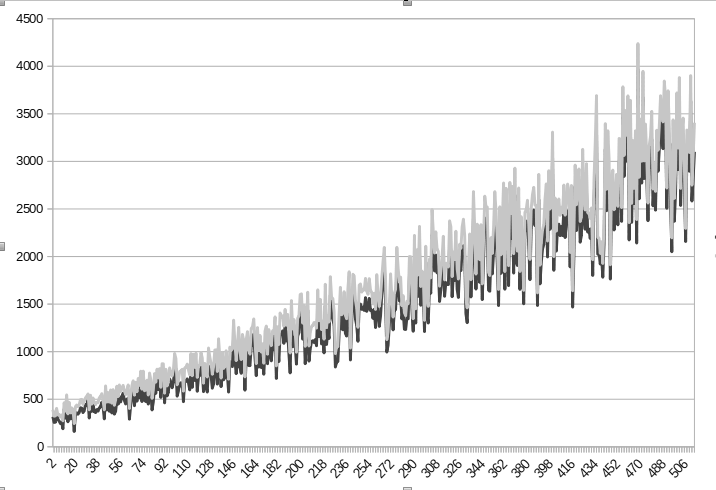
\includegraphics[width=80mm]{comparison_chart}
\end{figure}

One can see that completely meaningful encoding neatly trails DER, and
even is slightly more compressed (average overhead of DER to meaningful
encoding in this range is 13\%).

\subsection{DER Comparison - String Encoding}

\subsubsection{Method}

A JSON file was created, with a single key/value pair, where the value
is a string of increasing length (value of the X-axis times four).
The JSON was then fed to both the DER
encoder and the meaningful encoder. The resulting sizes of the binary were
then compared.

\subsubsection{Outcome}

\begin{figure}[H]
\centering
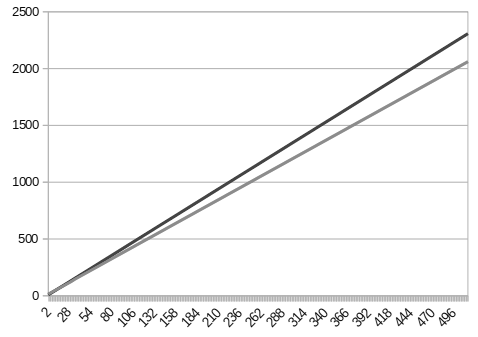
\includegraphics[width=80mm]{stringcomparison}
\end{figure}

It can be clearly seen that the DER encoding of strings is more
frugal than meaningful encoding (as expected). This should tend to
12.5\% (as can be seen from the graph).

\subsection{DER Comparison - Conclusion}

As expected, DER performs better at leaf (string) encoding while
meaningful encoding performs better at structural encoding.
The overhead percentages wrt one another seem to cancel each other
out statistically. Since this is so, a further expectation is that, with string
and integer encoding optimization as proposed in this paper implemented,
this balance could made more favourable of meaningful encoding.

\section{Examples}

\textit{
Binary data representations can be given in two formats, bit-wise and byte-wise.
Bit-wise data is preceeded, per section, by a 'B:',
while byte-wise data is preceeded, per section, by a 'H:' (and is denoted in
hexadecimal tuplets).
}

\subsection{Example 001}

The following input:

\begin{changemargin}{-60mm}{0mm}
\begin{myquote}
\begin{verbatim}

B: 0 0 0 0  0 0 0 0

\end{verbatim}
\end{myquote}
\end{changemargin}

Produces the following JSON:

\begin{changemargin}{-60mm}{0mm}
\begin{myquote}
\begin{verbatim}

[ ]

\end{verbatim}
\end{myquote}
\end{changemargin}

Three implicit nulls are read from the input, which are all discarded.
Since the implicit top-list now contains zero elements, it is presented
as the result of the decoding.

\subsection{Example 002}

The following input:

\begin{changemargin}{-60mm}{0mm}
\begin{myquote}
\begin{verbatim}

B: 0 0 1 0  0 0 0 0

\end{verbatim}
\end{myquote}
\end{changemargin}

Produces the following JSON:

\begin{changemargin}{-60mm}{0mm}
\begin{myquote}
\begin{verbatim}

null

\end{verbatim}
\end{myquote}
\end{changemargin}

An explicit null is read, followed by the read of two implicit nulls.
The implicit nulls are discarded (because they are in the tail).
Since the implicit top-list only contains one element, it is presented
as a single null, not encapsulated in an array.

\subsection{Example 003}

The following input:

\begin{changemargin}{-60mm}{0mm}
\begin{myquote}
\begin{verbatim}

B: 0 0 1 0  0 1 0 0

\end{verbatim}
\end{myquote}
\end{changemargin}

Produces the following JSON:

\begin{changemargin}{-60mm}{0mm}
\begin{myquote}
\begin{verbatim}

[ null, null ]

\end{verbatim}
\end{myquote}
\end{changemargin}

Here, two explicit (un-erasable) nulls are encoded in the implicit
top-list, followed by two zero bits. The decoder reads these bits
(and one more, which will also be virtually zero), and interprets that
as an implicit null. The implicit null is then discarded.

\subsection{Example 004}

The following input:

\begin{changemargin}{-60mm}{0mm}
\begin{myquote}
\begin{verbatim}

B: 1 1 0 1  0 0 0 0

\end{verbatim}
\end{myquote}
\end{changemargin}

Produces the following JSON:

\begin{changemargin}{-60mm}{0mm}
\begin{myquote}
\begin{verbatim}

[ null ]

\end{verbatim}
\end{myquote}
\end{changemargin}

In this example, the type number six (1 1 0) denotes an explicit array.
It is followed by a one-byte, which denotes the fact that the array
contains at least one more element. The subsequent zeroes denote the filling.

Note that the encoding could have also used an explicit null here
(making for 1 1 0 1  0 0 1 0).

\subsection{Example 005}

The following input:

\begin{changemargin}{-60mm}{0mm}
\begin{myquote}
\begin{verbatim}

B: 1 1 0 1  0 0 1 1    0 0 1 0  0 0 0 0

\end{verbatim}
\end{myquote}
\end{changemargin}

Read from left to right:
\begin{itemize}
\item 'I have a list' (3 bits).
\item 'The list has one more element' (1 bit).
\item 'I have an explicit null' (3 bits).
\item 'The list has one more element' (1 bit).
\item 'I have an explicit null' (3 bits).
\item 'The list has no more elements' (1 bit).
\item .. followed by zero bits which may be interpreted as implicit
      nulls, but which will be discarded.
\end{itemize}

Produces the following JSON:

\begin{changemargin}{-60mm}{0mm}
\begin{myquote}
\begin{verbatim}

[ null, null ]

\end{verbatim}
\end{myquote}
\end{changemargin}

Note that this is the exact same output as given in example 3, but now
made explicit.

\subsection{Example 006}

The following JSON input:

\begin{changemargin}{-60mm}{0mm}
\begin{myquote}
\begin{verbatim}

[
  "foo", "bar", { "foo" : "bar" }, [], [ [ ] ]
]

\end{verbatim}
\end{myquote}
\end{changemargin}

When encoded, leads to the following binary:

\begin{changemargin}{-60mm}{0mm}
\begin{myquote}
\begin{verbatim}

00000000  db 66 b7 db db 62 b0 dc  9f b3 5b ed eb 62 b0 dc  |.f...b....[..b..|
00000010  8e 77 00                                          |.w.|
00000013

\end{verbatim}
\end{myquote}
\end{changemargin}

Which, in turn, when fed to the decoder, leads to this JSON:

\begin{changemargin}{-60mm}{0mm}
\begin{myquote}
\begin{verbatim}

["foo","bar",{"foo":"bar"},[],[[]]]

\end{verbatim}
\end{myquote}
\end{changemargin}

For context: the same structure, more or less (DER has no concept of name/value
pair lists or hashtables), encoded as DER (10 more bytes required):

\begin{changemargin}{-60mm}{0mm}
\begin{myquote}
\begin{verbatim}

30 1c 04 03 f  o  o  04  03 b  a  r  30 0a 04 03 f  
o  o  04 03 b  a  r  30  00 30 02 30 00

\end{verbatim}
\end{myquote}
\end{changemargin}

